
\begin{figure}[!t]
    \centering
    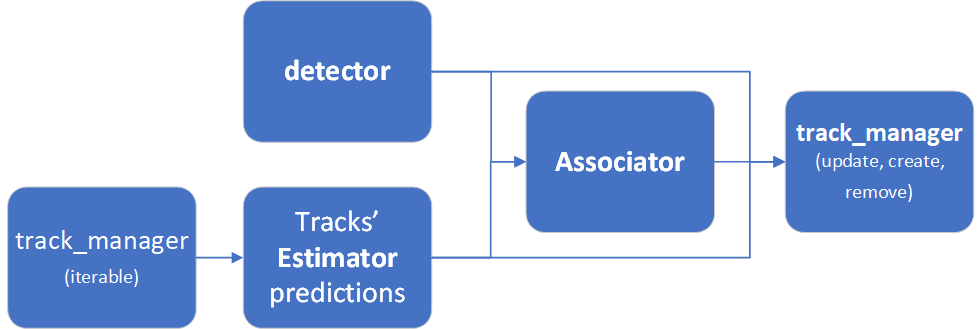
\includegraphics[width=0.9\linewidth]{figures/04_state_of_the_art/SORT.png}
    \caption[SORT algorithm]{\footnotesize{Block diagram of the SORT algorithm.}}
    \label{fig:sort}
    %\vspace{-1em}
\end{figure}

{
    \ac{SORT}\cite{Bewley2016_sort} is a model published in 2016, it reached competitive accuracies and speed simultaneously. 
    As it can be seen from the block diagram of the figure \ref{fig:sort}, the authors propose to use a system with the following four components:
}

\begin{enumerate}
    \item \textbf{Detector}: The detector solves the problem of finding an undefined number of regions that fit with a set of target objects within an image (frame). 
    The authors of \ac{SORT} use a \ac{CNN} based model that yields better detections than previous models, this reduce the estimations noise.
    \item \textbf{Estimator}: The estimator employs a Kalman filter, a recursive filter, to estimate the movement of each individual object based on noisy observations.
    \item \textbf{Associator}: The associator resolves the matching of the current frame detections with the active tracks estimations. The usage of a \ac{IoU} distance matrix and the Hungarian algorithm improved the speed with respect other systems.
    \item \textbf{Track manager}: The track manager creates and deletes the tracks given the other components results.
\end{enumerate}

%\needspace{0.1\textheight}

\paragraph{Detector}

{
    An operation that, given an input image, returns a set of output vectors containing the confidence, the object position, the object dimension and the class probability.
}

%\begin{equation}
%    \label{eqn:Detector definition}
%    Detector(I) = \{b_{0}, b_{1}, \hdots, b_{n}\} \; with \; b_{n} = \begin{bmatrix}
%        c \\
%        x \\
%        y \\
%        h \\
%        w \\
%        p_{c}
%      \end{bmatrix}
%\end{equation}
%
%\needspace{0.1\textheight}

\paragraph{Estimator}

{
    The \textbf{Kalman filter}\cite{kalman1960} operates in two main steps: prediction and updating.
    The prediction step estimates the \textbf{state mean} $x$ and covariance matrix $\mathbf{P}$ with the state transition matrix $\mathbf{F}$ and the process noise matrix $\mathbf{Q}$:
}
\begin{equation}
    \label{eqn:Kalman state mean estimation}
    \hat{x}_{k} = \mathbf{F} \cdot x_{k-1}
%    \hat{x}_{k} = \mathbf{F} \cdot x_{k-1} \; \; with \; x = \begin{bmatrix}
%        u \\
%        v \\
%        s \\
%        r \\
%        \dot u \\
%        \dot v \\
%        \dot s
%      \end{bmatrix}
\end{equation}

\begin{equation}
    \label{eqn:Kalman covariance matrix estimation}
    \hat{\mathbf{P}}_{k} = \mathbf{F} \cdot \mathbf{P}_{k-1} \cdot \mathbf{F}^{T} + \mathbf{Q}
\end{equation}

%{
%    Where $u \; and \; v$ is the object center, $s$ is the object scale, $r$ is the object aspect ratio and $\dot u, \dot v \; and \; \dot s$ are their velocities.
%}

{
    And, the updating step requires an observation $z$ (modified detection matched by the associator) 
    to correct the estimated state mean $x$ and covariance matrix $\mathbf{P}$ which improves the following iterations. 
    This is done with the Kalman gain $\mathbf{K}$, the measurements mask $\mathbf{H}$ and the measurements uncertainty matrix $\mathbf{R}$:
}

\begin{equation}
    \label{eqn:Kalman gain}
    \mathbf{K} = \hat{\mathbf{P}}_{k} \cdot \mathbf{H}^{T} \cdot (\mathbf{H} \cdot \mathbf{P}_{k} \cdot \mathbf{H}^{T} + \mathbf{R})^{-1}
\end{equation}

\begin{equation}
    \label{eqn:Kalman state mean correction}
    x_{k} = \hat{x}_{k} + \mathbf{K} \cdot (z - \mathbf{H} \cdot \hat{x}_{k})
%    x_{k} = \hat{x}_{k} + \mathbf{K} \cdot (z - \mathbf{H} \cdot \hat{x}_{k}) \; \; with \; z = \begin{bmatrix}
%        u\\ 
%        v\\ 
%        s\\ 
%        r
%        \end{bmatrix}
\end{equation}

\begin{equation}
    \label{eqn:Kalman covariance matrix correction}
    \mathbf{P}_{k} = (\mathbf{K} \cdot \mathbf{H})^{-1} \cdot \hat{\mathbf{P}}_{k} \cdot (\mathbf{K} \cdot \mathbf{H})^{-T} + \mathbf{K} \cdot \mathbf{R} \cdot \mathbf{K}^{T}
\end{equation}

\needspace{0.1\textheight}

\paragraph{Associator}

{
    The associator defines a \textbf{cost matrix} using negative \ac{IoU} between detections and estimations, with \ac{IoU} values below a certain threshold being rejected.
}

\begin{equation}
    \label{eqn:IoU}
    \begin{gathered}
        IoU(A, B) = \frac{|A \cap B|}{|A \cup B|} \\[0.25cm]
%        |A \cap B| = max(min_{x2}(A, B) - max_{x1}(A, B), 0) \cdot max(min_{y2}(A, B) - max_{y1}(A, B), 0) \\[0.25cm]
%        |A \cup B| = Area(A) + Area(B) - |A \cap B|
    \end{gathered}
\end{equation}

\needspace{0.1\textheight}

{
    The \textbf{Hungarian algorithm} associate the rows and columns assigning at most one row to each column and at most one column to each row with the minimum cost. 
    At the end, 3 sets are defined:
}

\begin{subequations}
    \begin{align}
        \mathit{A} = \{ (row, col) \mid (row, col) &\text{ is in the output of } Hungarian(-\mathbf{IoU}) \}
        \label{eqn:Assigned set} \\[0.5cm]
        \mathit{B} = \{ row &\mid \forall \: col \; \nexists \: (row, col) \in A \}
        \label{eqn:Unassigned detections set} \\[0.5cm]
        \mathit{C} = \{ col \mid& \; \forall \: row \; \nexists \: (row, col) \in A \}
        \label{eqn:Unassigned tracks set}
    \end{align}
\end{subequations}

\paragraph{Track manager}
{
    The Track Manager component uses the set of matched tracks and detections ($\mathit{A}$ in equation \ref{eqn:Assigned set}) 
    to update the Kalman filter for each assigned detection and track. 
    It also creates new potential tracks from unmatched detections ($\mathit{B}$ in equation \ref{eqn:Unassigned detections set}) 
    and potentially terminates tracks with missing associations ($\mathit{C}$ in equation \ref{eqn:Unassigned tracks set}).
}

{
    This model is the basis for subsequent tracking models discussed in this section.
}
